\documentclass{sdxxpaper}
\papertitle{基于 Transformer 的中文短文本摘要生成方法研究与实现}
\college{计算机科学与工程学院}
\major{}
\classnumber{}
\authorname{}
\studentid{}
\reportyear{}
\reportmonth{}

\begin{document}
\makecover
\cqutBeginReportBody
\zihao{5}
\setstretch{1.05}
\setlength{\emergencystretch}{2em}
\makepaperheading
\begin{center}
  \makepaperauthor\par
  {\small 重庆理工大学计算机科学与工程学院，重庆}
\end{center}

\paperabstract{针对中文资讯阅读成本较高的问题，本文研究基于预训练 BART 的中文短文本摘要生成方法。采用 LCSTS 数据整理版本，在不同训练数据规模下微调模型，并与原文截取和 TextRank 方法进行比较。使用字符级 ROUGE 及生成案例评价摘要质量。实验结果与结论：\textbf{【待训练完成后填写】}。}
\paperkeywords{中文文本摘要；Transformer；BART；预训练模型；ROUGE}
\begin{center}\textbf{Chinese Short-Text Summarization with Transformer-based Models}\end{center}
\noindent\textbf{Abstract:} This paper studies Chinese news summarization using pretrained BART. Models trained with different amounts of LCSTS data are compared with lead-30 and TextRank baselines using character-level ROUGE and case analysis. Results and conclusions: \textbf{[To be completed after the experiments.] }\\
\noindent\textbf{Keywords:} Chinese summarization; Transformer; BART; TextRank; ROUGE


\section{引言}
互联网平台持续产生大量中文资讯。读者常通过标题和简短介绍判断是否阅读全文；当信息量增长时，人工筛选与整理摘要的成本也随之上升。自动摘要旨在从文本中提炼主要内容并形成较短表达，可用于资讯聚合、检索结果和内容预览。

摘要方法通常分为抽取式和生成式。抽取式方法从原文选取句子或片段，结果容易追溯，但受原文位置及表达方式约束。直接截取开头计算成本低，却可能只保留背景而遗漏后文的关键数量或结论。生成式方法能够压缩和重组信息，但可能产生与原文不一致的实体、数字和因果关系，因此需要同时评价文本重合和事实正确性。

Transformer 利用注意力机制建立序列内部及输入输出之间的关联\cite{transformer}。BART 在编码器—解码器结构上通过重建受扰动文本进行预训练，适合迁移到摘要任务\cite{bart}。本文以中文短资讯为场景，使用 LCSTS 数据整理版本，在预训练中文 BART 上进行全参数微调，并比较截取基线、不同训练规模和解码方式。本文结合生成结果分析模型的信息压缩能力及事实错误，讨论实验边界和后续改进方向。

资讯摘要不仅需要保留事件主体和动作，还需要交代数量、时间等限定信息。标题式参考摘要经常将多个事实压缩到一个短句中，因此摘要系统必须同时处理内容选择与语言组织。本文将原文前 30 字作为低成本的位置基线，将句子排序方法作为抽取式对照，再与生成模型比较，以观察不同信息选择方式对摘要质量的影响。

\section{数据与方法}
\subsection{数据来源与划分}
LCSTS 是面向中文短文本摘要的数据集\cite{lcsts}。本文使用整理版本 \texttt{aligeniewcp22}/LCSTS，数据版本与获取方式见项目 README。该版本提供训练数据、有标签验证数据和公开测试数据；其说明指出，有标签验证数据保留人工评分为 3 至 5 的样本\cite{dataset}。

计划的数据预处理包括检查原文及参考摘要非空、去除两端空白，以及将每条记录转换为统一格式。先用随机种子 42 打乱有标签验证数据，再按原文去重，从中选取 1\,000 条验证样本和 725 条自划分测试样本。训练集抽样前排除与这两部分原文完全相同的记录，从原训练集采用蓄水池抽样得到 10\,000 条，再从中抽取 2\,000 条。两组训练集共用验证集与自划分测试集，2K 训练集是 10K 的子集。验证集用于选择模型，自划分测试集用于方法比较。

由于所用整理版本的公开测试文件没有参考摘要，本文从有标签验证数据中划分自划分测试集，用于各方法的统一比较。正式实验应核对训练、验证和测试数据之间的原文是否重复，并记录检查结果。

实验计划在两组模型中使用一致的数据划分，以便比较训练规模。训练样本的原文如果与验证或测试样本完全一致，会使模型可能直接记住文本，因此抽样前先排除完全相同的原文。相近事件的改写仍可能出现在不同集合，后续评价需要进一步检查。验证集用于选择训练轮次，自划分测试集用于统一比较各方案，二者承担不同任务。

\subsection{模型结构}
给定原文序列 $X=(x_1,\ldots,x_n)$ 和摘要序列 $Y=(y_1,\ldots,y_m)$，摘要生成可表示为条件序列生成问题：
\begin{equation}
P(Y\mid X)=\prod_{t=1}^{m}P(y_t\mid y_{<t},X).
\end{equation}
本文使用公开的 \texttt{OpenMOSS-Team/bart-base-chinese} 预训练模型\cite{model}，其编码器和解码器各有 6 层，隐藏层维度为 768，每层注意力有 12 个头。原文经分词并映射为向量后，编码器通过双向自注意力和前馈网络形成上下文表示；解码器根据已生成词元，通过交叉注意力读取编码器输出，逐步预测下一个词元。

注意力根据查询 $Q$ 和键 $K$ 的相似程度对值 $V$ 加权。缩放点积注意力为：
\begin{equation}
\operatorname{Attention}(Q,K,V)=\operatorname{softmax}\!\left(\frac{QK^{T}}{\sqrt{d_k}}\right)V,
\end{equation}
其中 $d_k$ 为键向量维度\cite{transformer}。编码器自注意力建立原文词元之间的联系；解码器自注意力受因果掩码约束，只使用当前位置之前的词元；交叉注意力使生成过程利用原文表示。本文沿用预训练结构及权重，训练时以参考摘要监督词元预测，更新全部可训练参数，填充位置不参与损失计算，未增加额外网络支路。

模型所用分词器为 BertTokenizer：它先进行基本分词，再使用 WordPiece 词表拆分词元，中文字符会先单独切分，连续拉丁词串可拆分为子词。模型配置的解码器起始词元 ID 为 102；解码时以该词元作为初始输入，随后由已生成词元构成 $y_{<t}$。输入词元嵌入与可学习的位置嵌入相加，为注意力层提供顺序信息。编码器输出同时供解码器交叉注意力使用：查询来自解码器当前隐藏状态，键和值来自原文表示，由此在每一步为生成选择相关上下文。训练采用目标序列右移的教师强制方式，推理阶段则使用模型自身生成的历史。

\begin{figure}[htbp]
\centering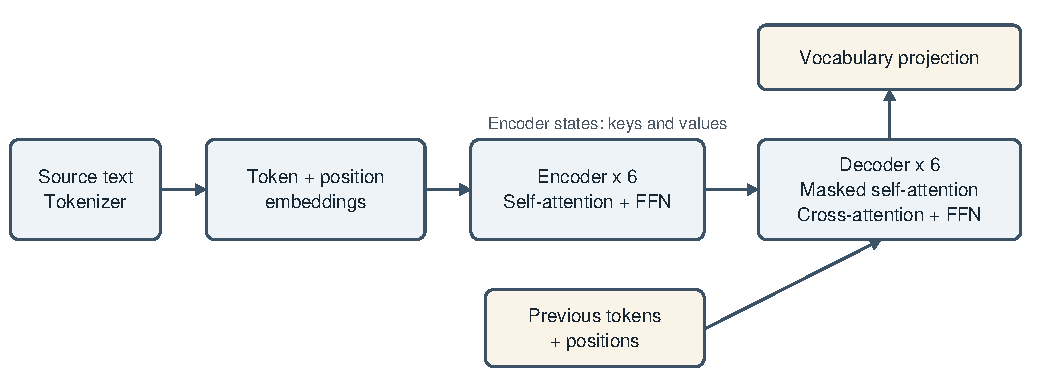
\includegraphics[width=0.92\linewidth]{assets/bart-architecture.pdf}
\caption{BART 编码器—解码器结构及摘要生成流程}\label{fig:architecture}
\end{figure}

图~\ref{fig:architecture} 中的结构是对预训练模型的任务化使用。编码器和解码器各包含六层，多头注意力在不同表示子空间计算权重，前馈网络对每个位置的表示作非线性变换。解码器的掩码防止训练时读取未来词元；交叉注意力则连接原文与输出，使生成的标题既利用历史摘要，也能从输入中选取事件信息。

\subsection{训练、解码与评价}
采用模型对应的分词器，原文和目标摘要长度上限分别为 128 和 32 token，超长部分截断，批内动态填充。两组模型均使用 AdamW，初始学习率 $3\times10^{-5}$，线性衰减、不预热，批大小为 4，训练 3 轮，随机种子为 42。每轮结束计算验证损失，选取损失最低的模型生成摘要。实际实验设备、软件版本及运行环境：\textbf{【待填写】}。

计划对照包括原文前 30 字截取、TextRank 抽取，以及 2K 和 10K 模型分别使用贪心搜索与束搜索。贪心搜索每步只保留当前概率最高的词元；束搜索每步保留多个候选序列，本文束宽为 4。两种策略均关闭随机采样，最多生成 32 个新 token，输出时去除特殊词元和分词引入的空白。

TextRank 将句子作为图节点，根据内容相似度建立带权边并迭代更新节点得分\cite{textrank}。本实验按句号、问号、感叹号、分号及换行切分句子；以单个汉字及连续英文或数字串作为词元，英文统一小写。两句边权为词元多重集合重合数除以两句词元数分别加一后取对数之和。排序阻尼系数为 0.85，最多迭代 100 次，最大变化小于 $10^{-8}$ 时停止；无出边节点均匀分配权重。选得分最高的句子，同分取原文中较早者，再截取前 30 字。该实现保留可复现的简明规则，截断可能使输出成为片段。

本文使用去除空白后的字符级 ROUGE F1\cite{rouge}。ROUGE-$N$ 统计候选和参考中的字符 $N$ 元片段及其多重集合交集；分别以交集大小 $c$、候选片段数 $n_p$ 和参考片段数 $n_r$ 计算精确率与召回率。ROUGE-L 则以最长公共子序列长度作为 $c$，以候选和参考的字符数作为分母。两类指标均按下式计算，并先逐样本计算再取算术平均：
\begin{equation}
P=\frac{c}{n_p},\quad R=\frac{c}{n_r},\quad F_1=\frac{2PR}{P+R}.
\end{equation}
当候选或参考为空、无重合，或 $P+R=0$ 时，按实现将该样本的 F1 记为零。ROUGE 衡量与参考文本的表面重合，事实关联还需结合输入原文检查。

\section{实验与结果}
\subsection{验证损失与模型选择}
完成模型训练后，填写每轮验证损失及所选轮次，并根据训练日志生成损失曲线。选择模型时以验证集损失为准。
\begin{figure}[htbp]
\centering\fbox{\parbox[c][3.2cm][c]{0.85\linewidth}{\centering 训练与验证损失曲线【待填写】}}
\caption{训练与验证损失曲线}\label{fig:loss}
\end{figure}
\begin{table}[htbp]
\centering\caption{各轮验证损失与选中轮次}\label{tab:loss}
\renewcommand{\arraystretch}{1.2}
\begin{tabular}{lcccc}\toprule
训练样本数 & 第 1 轮 & 第 2 轮 & 第 3 轮 & 选中轮次\\\midrule
2\,000 & 待填写 & 待填写 & 待填写 & 待填写\\
10\,000 & 待填写 & 待填写 & 待填写 & 待填写\\\bottomrule
\end{tabular}
\end{table}
\noindent\textbf{训练与验证损失分析：【待填写】}

\subsection{摘要生成性能与解码策略比较}
在相同测试集上计算字符级 ROUGE，并分别记录各方法的输出长度与生成耗时。表中数值及结果分析均在实验完成后填写；计时应注明运行设备和是否包含模型加载。
\begin{table}[htbp]
\centering\caption{不同方法在自划分测试集上的结果}\label{tab:results}
\renewcommand{\arraystretch}{1.2}
\begin{tabular}{lccccc}\toprule
方法 & R-1 & R-2 & R-L & 平均长度 & 耗时/s\\\midrule
前 30 字 & -- & -- & -- & -- & --\\
TextRank & -- & -- & -- & -- & --\\
BART 2K，贪心搜索 & -- & -- & -- & -- & --\\
BART 2K，束搜索 & -- & -- & -- & -- & --\\
BART 10K，贪心搜索 & -- & -- & -- & -- & --\\
BART 10K，束搜索 & -- & -- & -- & -- & --\\\bottomrule
\end{tabular}
\end{table}
\noindent\textbf{基线与数据规模比较：【待填写】}\par
\noindent\textbf{贪心搜索与束搜索比较：【待填写】}

\subsection{典型案例分析}
选择具有代表性的测试样本，逐项列出完整原文、参考摘要和各方法的输出，再讨论关键信息、数字和事件关系。
\begin{table}[htbp]
\centering\caption{摘要生成案例【待填写】}\label{tab:case}
\begin{tabularx}{\linewidth}{@{}>{\raggedright\arraybackslash}p{6em}X@{}}\toprule
原文 & 【待填写】\\
参考摘要 & 【待填写】\\
前 30 字 & 【待填写】\\
TextRank & 【待填写】\\
2K 贪心搜索 & 【待填写】\\
2K 束搜索 & 【待填写】\\
10K 贪心搜索 & 【待填写】\\
10K 束搜索 & 【待填写】\\\bottomrule
\end{tabularx}
\end{table}
\noindent\textbf{案例分析：【待填写】}

\section{分析与讨论}
\subsection{实验结果分析}
\noindent\textbf{数据规模、训练过程与生成质量的关系：【待填写】}\par
\noindent\textbf{不同解码策略与基线方法的比较：【待填写】}\par
\noindent\textbf{事实一致性与典型错误分析：【待填写】}

ROUGE 可用于衡量输出与参考摘要的字符重合，但不能单独判断数字、实体和事件之间的对应关系。案例分析应结合完整原文检查摘要是否准确表达事件，并区分信息遗漏和事实错误。

\subsection{实验局限与改进方向}
本方案拟从有标签验证数据中划分验证集和自划分测试集；自划分测试集并非官方测试集。实际报告应记录数据来源、划分方法和测试集的使用情况，并说明随机种子、训练次数及可能存在的跨划分近似重复。进一步实验可考虑独立测试集、多个随机种子和人工事实性评价。

\section{总结}
\noindent\textbf{主要工作、实验结果与结论：【待填写】}

\begin{thebibliography}{99}
\bibitem{transformer} Vaswani A, Shazeer N, Parmar N, et al. Attention Is All You Need[C]//Advances in Neural Information Processing Systems 30. 2017: 5998--6008.
\bibitem{bart} Lewis M, Liu Y, Goyal N, et al. BART: Denoising Sequence-to-Sequence Pre-training for Natural Language Generation, Translation, and Comprehension[C]//ACL. 2020: 7871--7880. \url{https://aclanthology.org/2020.acl-main.703/}.
\bibitem{lcsts} Hu B, Chen Q, Zhu F. LCSTS: A Large Scale Chinese Short Text Summarization Dataset[C]//EMNLP. 2015: 1967--1972. \url{https://aclanthology.org/D15-1229/}.
\bibitem{dataset} aligeniewcp22. LCSTS 数据集说明[EB/OL]. \url{https://huggingface.co/datasets/aligeniewcp22/LCSTS/blob/main/README-ZH.md}.
\bibitem{model} OpenMOSS-Team. Chinese BART-Base 模型说明[EB/OL]. \url{https://huggingface.co/OpenMOSS-Team/bart-base-chinese}.
\bibitem{textrank} Mihalcea R, Tarau P. TextRank: Bringing Order into Text[C]//Proceedings of EMNLP. 2004: 404--411. \url{https://aclanthology.org/W04-3252/}.
\bibitem{rouge} Lin C Y. ROUGE: A Package for Automatic Evaluation of Summaries[C]//Text Summarization Branches Out. 2004: 74--81. \url{https://aclanthology.org/W04-1013/}.
\end{thebibliography}
\end{document}
